\section{\textbf{Introduction}}\label{sec:Introduction}
Adaptive streaming video standards are the norm for anything that is video and is streamed over the internet nowadays
For streaming adaptive video there are two main standards, MPEG-DASH and Apple‘s HLS – both similar in how they work
Instead of a single video file being transferred to clients, adaptive streaming works by splitting video into smaller segments, each segment being its own file. These video segment files are referenced by playlist files that specify time, duration and order of segments
By providing playlists and video segments playback becomes much more flexible and robust as it provides a number of benefits
Splitting of video and audio tracks, to e.g. provide multiple different audio tracks with different languages
Provide multiple video tracks with different resolution and bitrate to accomodate (temporary) bandwith bottlenecks during transfer
Being able to seamlessly switch between tracks to e.g. 720p, 1080p or 4K video resolution

\begin{figure}

\centering
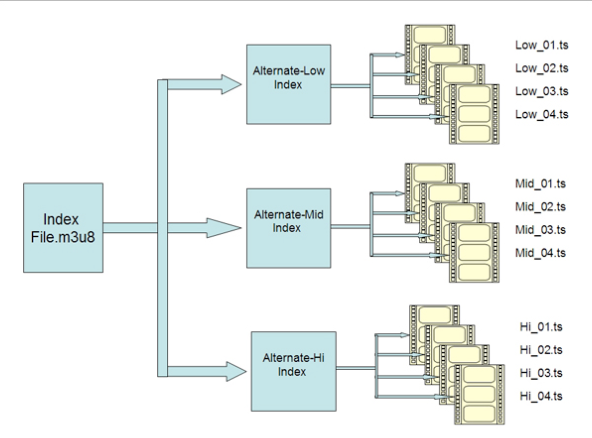
\includegraphics[scale=0.40]{figures/ProblemStatement.png}
\caption{Problem Statement \cite{rancy2016imt}}
\label{fig:IMT_2020_Use-cases}
\end{figure}


\subsection{Problem Statement
}\label{Problem Statement
}

We are in the Streaming Era

Content is transmitted without downloading

ABS dynamically changes the video source to avoid buffering

HLS splits a video file into little segments 

Not all streams share the same representations

We need an algorithm that identifies matching representation from variant video streams in order to output a single playlist











